% Figura Anexo III: cronología de la nueva macroeconomía clásica (1961-1988): aportaciones arriba, contexto abajo
\documentclass[tikz,border=3pt]{standalone}
\usepackage[T1]{fontenc}
\usepackage[utf8]{inputenc}
\usetikzlibrary{arrows.meta,calc,positioning}
\begin{document}
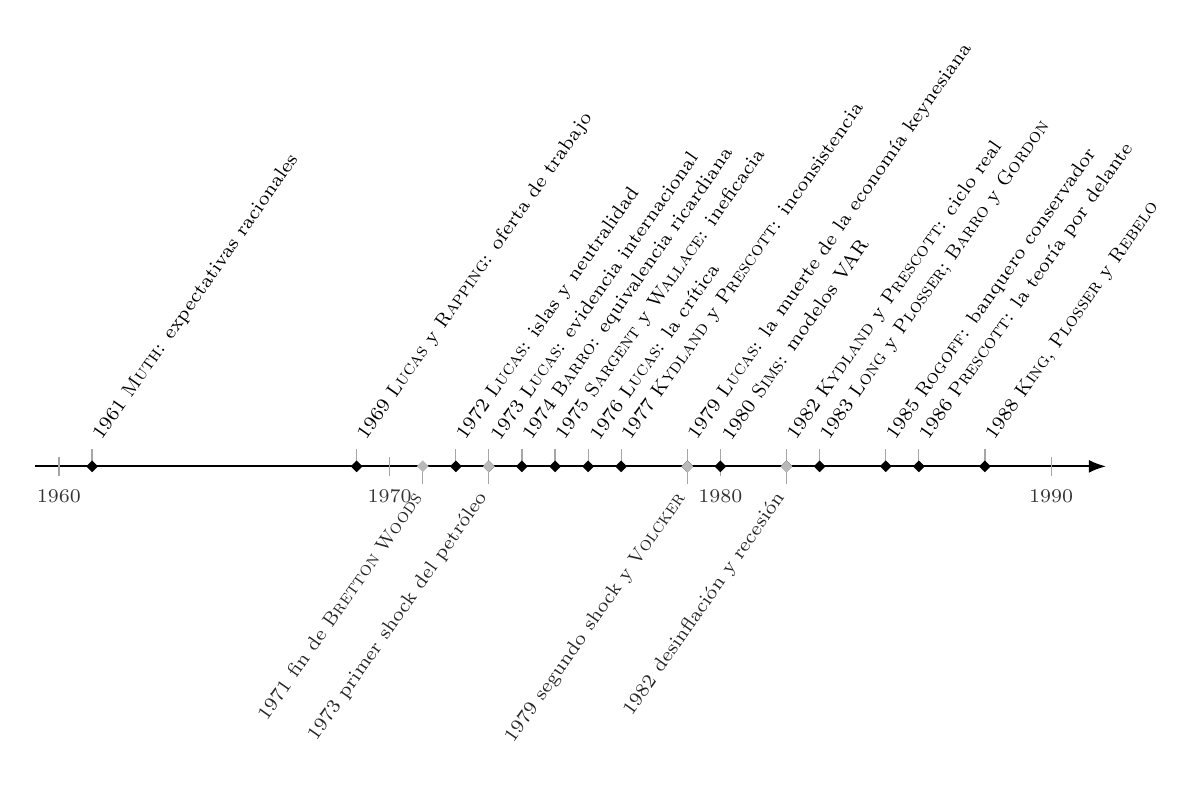
\begin{tikzpicture}[>={Latex[length=2.2mm]}, font=\footnotesize,
  hito/.style={rectangle, fill=black, inner sep=1.5pt, rotate=45},
  ctx/.style={rectangle, fill=gray!55, inner sep=1.5pt, rotate=45},
  arriba/.style={rotate=55, anchor=west, font=\scriptsize},
  abajo/.style={rotate=55, anchor=east, font=\scriptsize, gray!30!black},
  lead/.style={gray!70, thin}]
  % Eje
  \draw[->, thick] (-0.3,0) -- (13.3,0);
  \foreach \y in {1960,1970,1980,1990}{
    \pgfmathsetmacro{\x}{(\y-1960)*0.42}
    \draw[gray!70] (\x,-0.12) -- (\x,0.12);
    \node[font=\scriptsize, gray!40!black, anchor=north] at (\x,-0.18) {\y};
  }
  % Aportaciones (arriba)
  \foreach \y/\txt in {%
    1961/{1961 \textsc{Muth}: expectativas racionales},
    1969/{1969 \textsc{Lucas} y \textsc{Rapping}: oferta de trabajo},
    1972/{1972 \textsc{Lucas}: islas y neutralidad},
    1973/{1973 \textsc{Lucas}: evidencia internacional},
    1974/{1974 \textsc{Barro}: equivalencia ricardiana},
    1975/{1975 \textsc{Sargent} y \textsc{Wallace}: ineficacia},
    1976/{1976 \textsc{Lucas}: la crítica},
    1977/{1977 \textsc{Kydland} y \textsc{Prescott}: inconsistencia},
    1979/{1979 \textsc{Lucas}: la muerte de la economía keynesiana},
    1980/{1980 \textsc{Sims}: modelos VAR},
    1982/{1982 \textsc{Kydland} y \textsc{Prescott}: ciclo real},
    1983/{1983 \textsc{Long} y \textsc{Plosser}; \textsc{Barro} y \textsc{Gordon}},
    1985/{1985 \textsc{Rogoff}: banquero conservador},
    1986/{1986 \textsc{Prescott}: la teoría por delante},
    1988/{1988 \textsc{King}, \textsc{Plosser} y \textsc{Rebelo}}}{
    \pgfmathsetmacro{\x}{(\y-1960)*0.42}
    \draw[lead] (\x,0) -- (\x,0.22);
    \node[hito] at (\x,0) {};
    \node[arriba] at (\x,0.26) {\txt};
  }
  % Contexto (abajo)
  \foreach \y/\txt in {%
    1971/{1971 fin de \textsc{Bretton Woods}},
    1973/{1973 primer shock del petróleo},
    1979/{1979 segundo shock y \textsc{Volcker}},
    1982/{1982 desinflación y recesión}}{
    \pgfmathsetmacro{\x}{(\y-1960)*0.42}
    \draw[lead] (\x,0) -- (\x,-0.22);
    \node[ctx] at (\x,0) {};
    \node[abajo] at (\x,-0.26) {\txt};
  }
\end{tikzpicture}
\end{document}
